\documentclass[tikz,10pt]{standalone}

 \definecolor{ccred}{cmyk}{0, 0.87, 0.8, 0.21}
 \definecolor{cccanard}{RGB}{4,139,154}
 \definecolor{ccargile}{RGB}{239,239,239}

\begin{document}
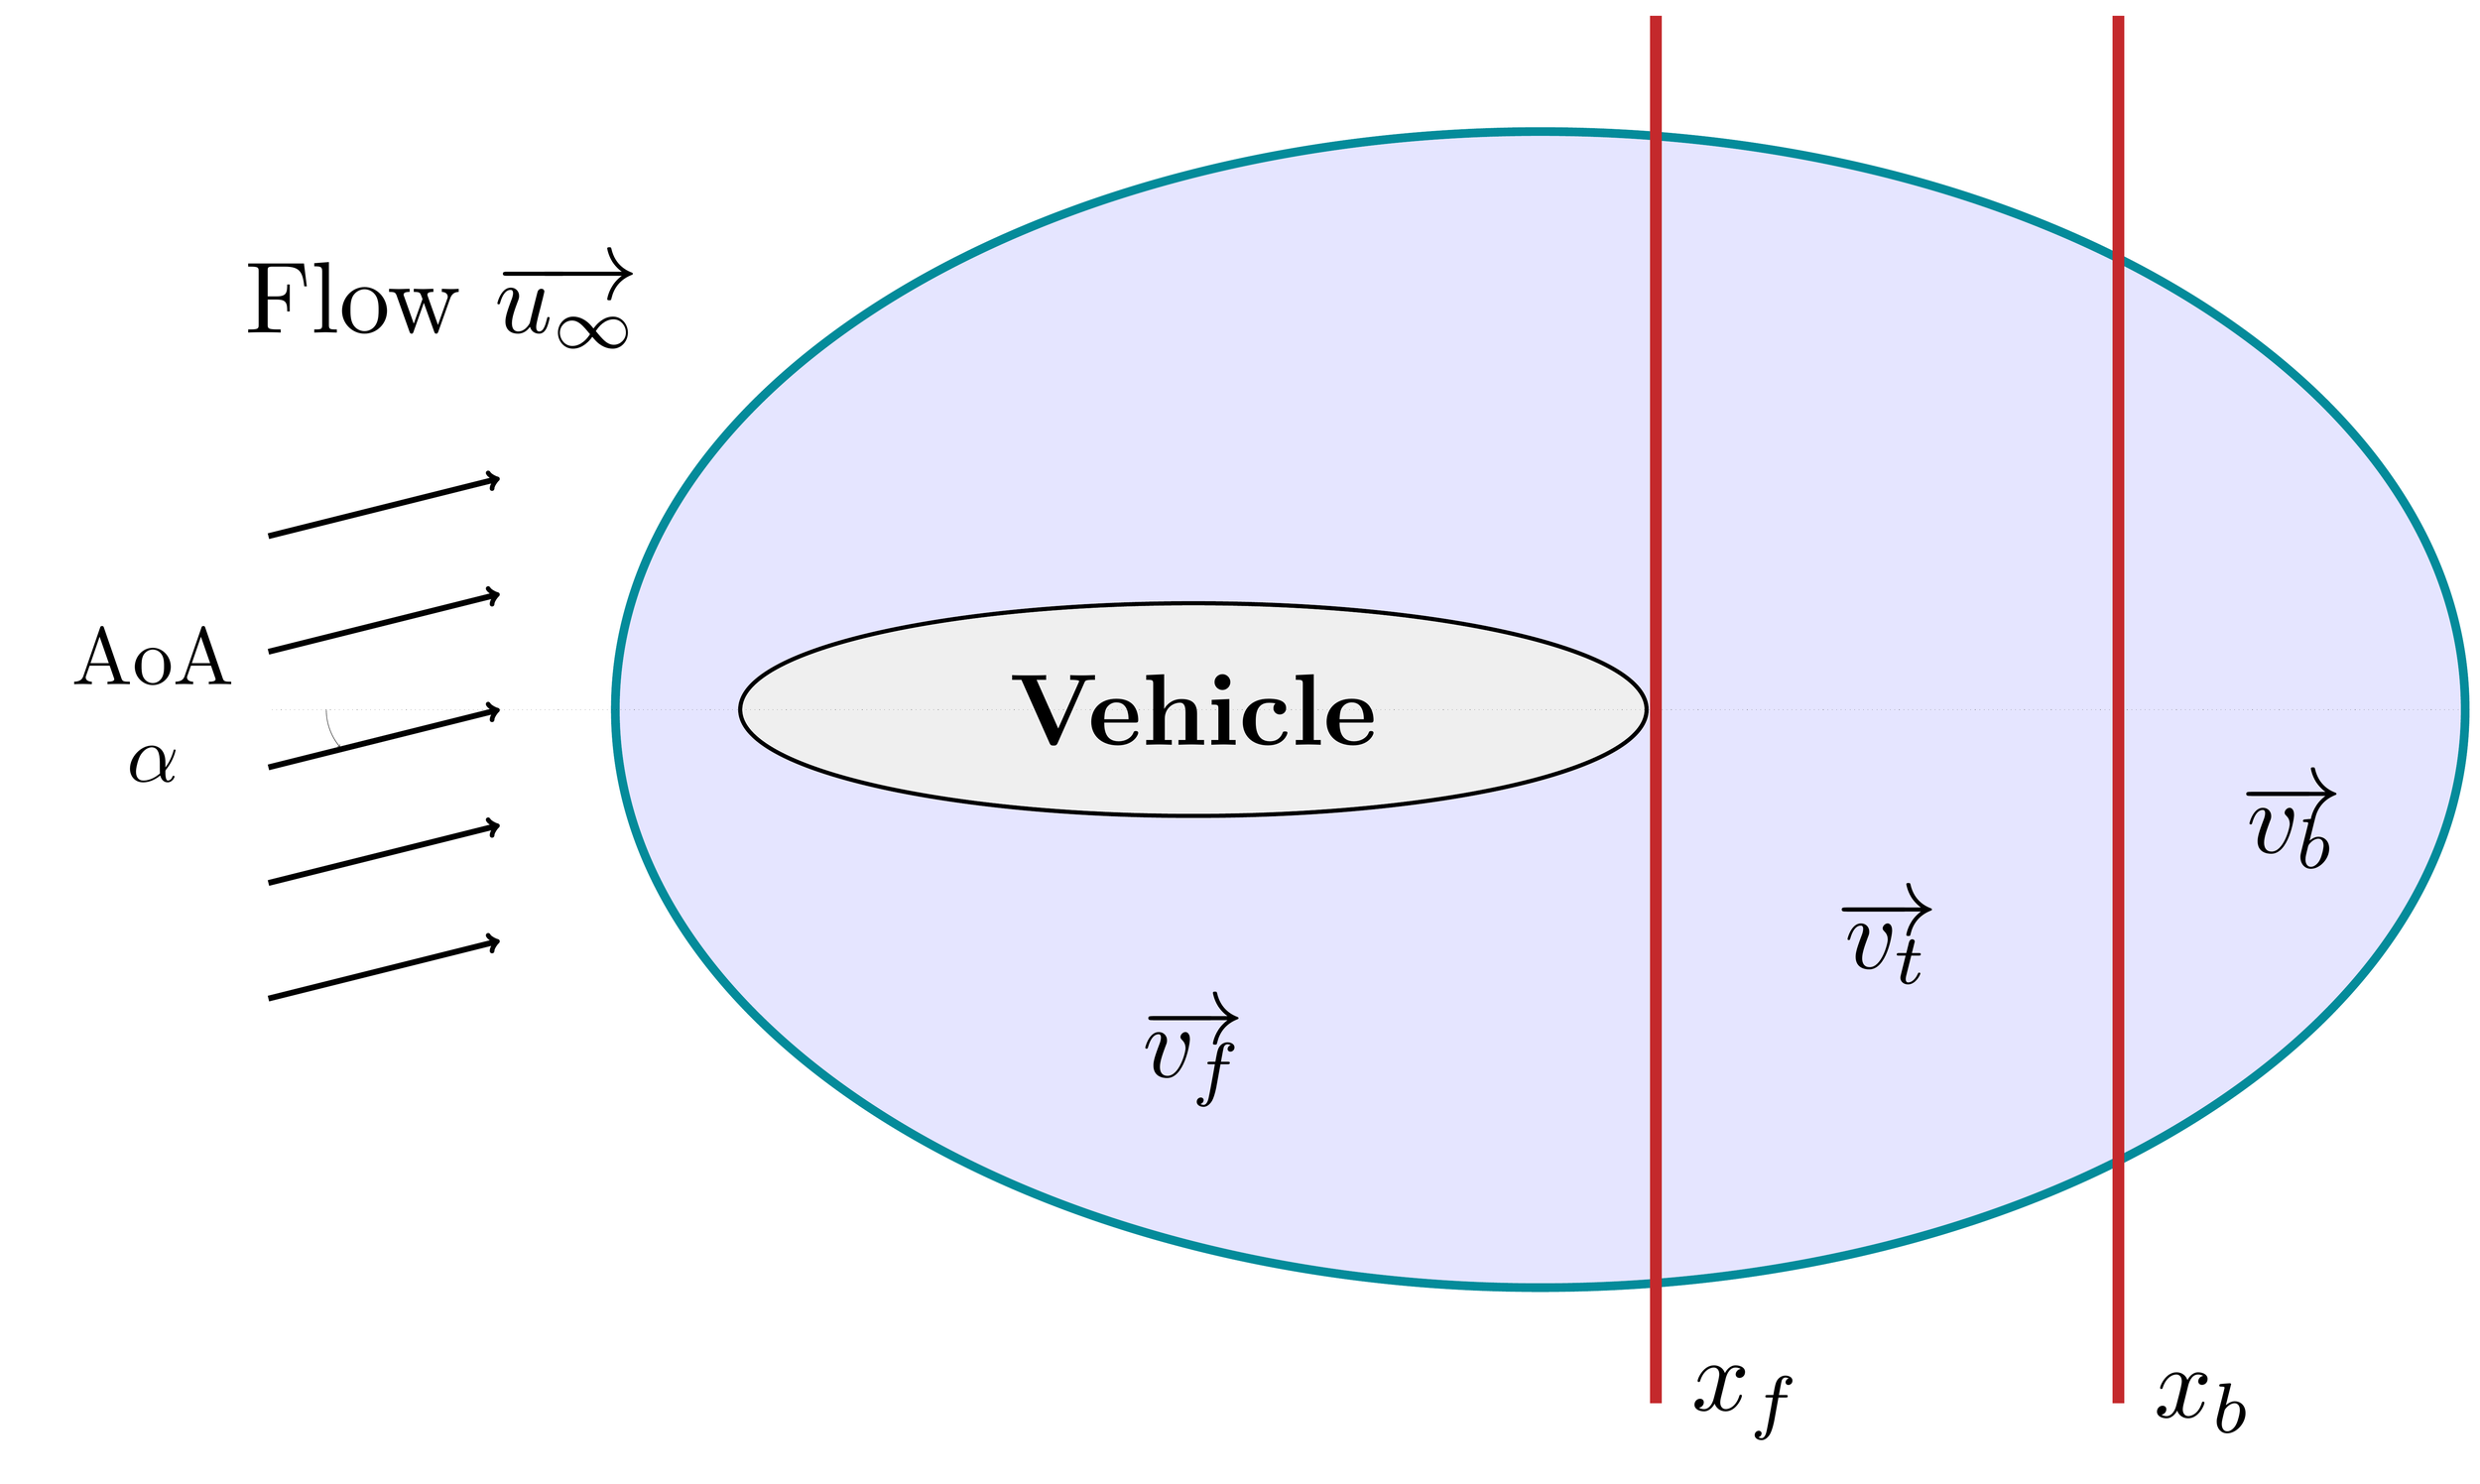
\begin{tikzpicture}[scale=4]

  % Flow
  \draw[fill=white!90!blue] (6,0) circle [x radius=8cm, y radius=5cm];

  % Vehicle
  \draw[fill=white, color=black, line width=3mm] (3,0) circle [x radius=3.9cm, y radius=0.9cm];
  \filldraw[fill=ccargile, color=ccargile] (3,0) circle [x radius=3.9cm, y radius=0.9cm];
  \draw(3,0) node[scale=10] (objet) {\textbf{Vehicle}};

  % Farfield
  \draw[line width=3mm, cccanard] (6,0) circle [x radius=8cm, y radius=5cm];

  % Amont
  \draw[->, line width=2mm] (-5,-2.5) -- (-3,-2);
  \draw[->, line width=2mm] (-5,-1.5) -- (-3,-1);
  \draw[->, line width=2mm] (-5,-0.5) -- (-3,0);
  \draw[->, line width=2mm] (-5,0.5) -- (-3,1);
  \draw[->, line width=2mm] (-5,1.5) -- (-3,2);
  \draw(-3.5,3.5) node[scale=10, black] (ecoulement) {Flow $\overrightarrow{u_\infty}$};

  % Axis
  \draw (-5,0) node (begin) {};
  \draw (14,0) node (end) {};
  \draw[loosely dotted] (begin) -- (end) ;

  % AoA (Angle of Attack)
  \draw (-5,-0.5) node (u1) {};
  \draw (-3, 0) node (u2) {};
  \draw[->] (-4.5,0) arc (180:220:0.5cm);
  \draw(-6,0.5) node[scale=8, black, text width=1cm] (AoA) {\begin{center} AoA $\alpha$ \end{center}};


  % Limites
  \draw[color=ccred, line width=4mm] (7,-6) -- (7,6) ;
  \draw[color=ccred, line width=4mm] (11,-6) -- (11,6) ;
  \draw (7,-6) node[scale=10, right] (xfront) {$x_{f}$};
  \draw (11,-6) node[scale=10, right] (xfront) {$x_{b}$};
  \draw (3,-3) node[scale=10] (xfront) {$\overrightarrow{v_{f}}$};
  \draw (9,-2) node[scale=10] (xfront) {$\overrightarrow{v_{t}}$};
  \draw (12.5,-1) node[scale=10] (xfront) {$\overrightarrow{v_{b}}$};
 

\end{tikzpicture}
\end{document}